\documentclass[12pt]{article}

\usepackage{graphicx}
\usepackage{indentfirst}
\usepackage[a4paper, total={6in, 8in}]{geometry}
\usepackage{hyperref}
\usepackage{fancyhdr}
\usepackage{xepersian}
\settextfont{B Nazanin}
\setlatintextfont{Times New Roman}

\begin{document}


%title page%
\begin{titlepage}
	\begin{center}
		\vspace{0.2cm}
		
		
\includegraphics[width=0.4\textwidth]{sharif.png}\\
		\vspace{0.2cm}
		\textbf{ \Huge{آشنایی با \lr{DHCP}}}\\
		\vspace{0.25cm}
		\textbf{ \Large{آز شبکه - دکتر بردیا صفایی}}
		\vspace{0.2cm}
		
		
		\large \textbf{دانشکده مهندسی کامپیوتر}\\\vspace{0.1cm}
		\large   دانشگاه صنعتی شریف\\\vspace{0.2cm}
		\large   ﻧﯿﻢ‌سال اول ۰۱-۰۲ \\\vspace{0.10cm}
		\large{ گروه 8:}\\
		\large{\href{mailto:mehrshad.mirmohammadi@gmail.com}{مهرشاد میرمحمدی - 98109634}}\\
		\large{\href{mailto:parhaamsaremi@gmail.com}{پرهام صارمی - 97101959}}\\
		\large{\href{mailto:mofayezi.m@gmail.com}{محمدرضا مفیضی - 98106059}}\\
	\end{center}
\end{titlepage}
%title page%

\newpage

%pages header
\pagestyle{fancy}
\fancyhf{}
\fancyfoot{}
\setlength{\headheight}{59pt}
\cfoot{\thepage}
\lhead{آشنایی با \lr{DHCP}}
\rhead{
\includegraphics[width=0.1\textwidth]{sharif.png}\\
		دانشکده مهندسی کامپیوتر
}
\chead{آز شبکه - گروه 8}
%pages header

\section*{مقدمه}
در این جلسه به معرفی پروتکل \lr{DHCP} \LTRfootnote{\lr{Dynamic Host Configuration Protocol}}  برای دریافت خودکار آدرس در شبکه می‌پردازیم.
\section{\lr{DHCP}}
\lr{DHCP} یک پروتکل کلاینت-سرور است که به طور خودکار برای یک میزبان پروتکل اینترنت (\lr{IP}) آدرس \lr{IP} و سایر اطلاعات پیکربندی مرتبط مانند ماسک زیر شبکه \LTRfootnote{\lr{subnet mask}} و دروازه پیش فرض \LTRfootnote{\lr{default gateway}} را فراهم می‌کند.
به عبارت دیگر، \lr{DHCP} به میزبان‌ها اجازه می‌دهد تا اطلاعات پیکربندی \lr{TCP/IP }مورد نیاز را از سرور \lr{DHCP} بدست آورند.

هر دستگاه در یک شبکه مبتنی بر \lr{TCP/IP} باید یک آدرس \lr{IP} منحصر به فرد برای دسترسی به شبکه و منابع آن داشته باشد. بدون \lr{DHCP}، آدرس‌های \lr{IP} رایانه‌های جدید یا رایانه‌هایی که از یک زیرشبکه به شبکه دیگر منتقل می‌شوند باید به صورت دستی پیکربندی شوند. آدرس‌های \lr{IP} رایانه‌هایی که از شبکه حذف می‌شوند هم باید به صورت دستی بازیابی شوند.

با \lr{DHCP}، کل این فرآیند به صورت خودکار و مرکزی مدیریت می‌شود. سرور \lr{DHCP} مجموعه‌ای از آدرس‌های \lr{IP} را نگه می‌دارد و هنگام راه‌اندازی در شبکه، آدرسی را به هر کلاینت فعال \lr{DHCP} می‌دهد. از آن‌جایی که آدرس‌های \lr{IP} به جای ثابت (به طور دائمی اختصاص داده‌شده) پویا هستند، آدرس‌هایی که دیگر استفاده نمی‌شوند به طور خودکار برای تخصیص مجدد به محموعه \lr{IP} بازگردانده می‌شوند.

برای راه‌اندازی یک سرور \lr{DHCP} باید ابتدا یک یا چند مخزن \LTRfootnote{\lr{pool}} \lr{IP} را تعریف کنیم. در \lr{IPv4} فرایند ارتباط دستگاه با سرور \lr{DHCP} شامل 4 مرحله است که در شکل \ref{fig:dhcp-session} نمایش داده شده است.

\begin{figure}[h!]
	\centering
	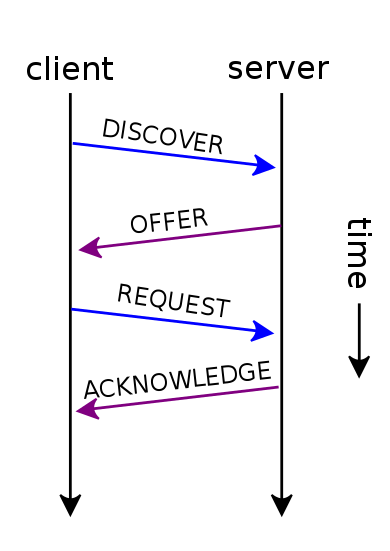
\includegraphics[width=0.3\columnwidth]{figs/DHCP_session.png}
	\caption{نمایشی از یک \lr{session} در پروتکل \lr{DHCP}}
	\label{fig:dhcp-session}
\end{figure}

\subsection{سناریو}
سناریو شکل \ref{fig:scenario} را در نظر بگیرید.
\begin{figure}[h!]
	\centering
	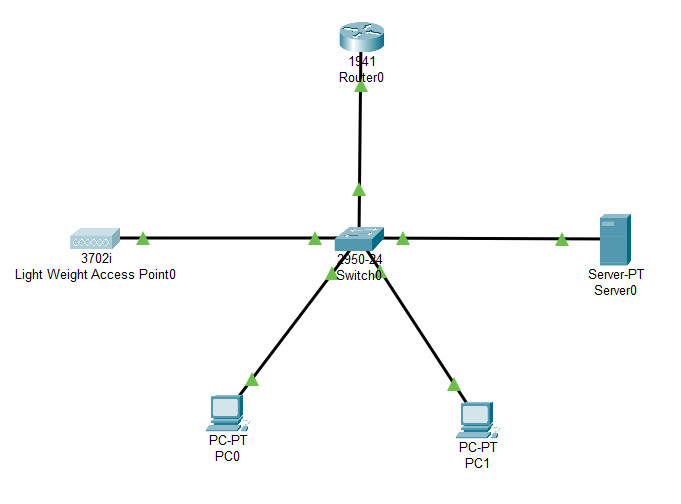
\includegraphics[width=0.5\columnwidth]{figs/s-1.jpg}
	\caption{سناریو مورد نظر}
	\label{fig:scenario}
\end{figure}
در این سناریو ما یک سرور برای سرویس \lr{DHCP}، دو \lr{PC}، یک
\lr{Light Weight Access Point}
و یک روتر به عنوان \lr{Gateway} در نظر می‌گیریم.
به منظور استفاده از \lr{DHCP} به \lr{PC}ها آدرسی نمی‌دهیم. 

ابتدا باید در سرور و رفتن به بخش \lr{Services} تنظیمات \lr{DHCP} و تعریف مخزن 
\lr{IP}
را انجام دهید. 
حالا می‌توانید با رفتن به یکی از \lr{PC}ها و انتخاب گزینه \lr{DHCP} در بخش
\lr{IP Configuration}
آدرس‌ها را دریافت کنید. همچنین می‌توانید در \lr{Light Weight Access Point} آدرس و مقدار \lr{primary controller} را با \lr{DHCP} دریافت کنید.

\subsection{سوال‌ها}
پس

\end{document}
